% elm-as-a-web-interface-development-language.tex
% Title: Elm как язык разработки веб-интерфейсов
% Author: Evgeny Simonenko <easimonenko@mail.ru>
% License: CC BY-ND 4.0

\documentclass[11pt,aspectratio=169]{beamer}

\usepackage[utf8x]{inputenc}
\usepackage[OT1]{fontenc}
\usepackage[english, russian]{babel}

\usetheme{Boadilla}

\usepackage{graphicx}
\graphicspath{{images/}}

\usepackage{listings}
\lstset{fontadjust=true}
\lstdefinelanguage{elm}
    {morekeywords={case,exposing,import,module,of,port,type},
    sensitive=true,
    morecomment=[l]{--},
    morestring=[b]"
    }

\begin{document}

\author{Симоненко Е.А. \\ \texttt{easimonenko@mail.ru}}
\title{Elm как язык разработки веб-интерфейсов}
\date{2018}

\begin{frame}
\titlepage
\end{frame}

\begin{frame}
\frametitle{Содержание}
\tableofcontents
\end{frame}

\section{Мотивация и история появления Elm}

\begin{frame}
\frametitle{Мотивация}
Требования:
\begin{itemize}
	\item функциональный
	\item статически типизированный
\end{itemize}
Варианты:
\begin{itemize}
	\item \textit{\texttt{GHCJS}} \url{https://github.com/ghcjs/ghcjs}
	\item \textit{\texttt{PureScript}} \url{http://www.purescript.org/}
	\item \textit{\texttt{Haste}} \url{https://haste-lang.org/}
	\item \textit{\texttt{Fay}} \url{https://github.com/faylang/fay/}
	\item \textit{\texttt{Idris}} \url{https://www.idris-lang.org/}
	\item \textit{\texttt{Elm}} \url{http://elm-lang.org/}
\end{itemize}
\end{frame}

\begin{frame}
\frametitle{История появления Elm}
\begin{itemize}
	\item 2012
	\item дипломная работа студента
	\item автор: Эван Чаплицкий (Evan Czaplicki)
	\item функционально-реактивный язык
\end{itemize}
\end{frame}

\begin{frame}
\frametitle{Как Haskell, только проще, и чтобы в браузере}
\begin{itemize}
	\item синтаксис как в Haskell
	\item отсутствуют классы типов, а заодно и монады
	\item компилируется в JavaScript для браузера
\end{itemize}
\end{frame}

\begin{frame}
\frametitle{Особенности}
\begin{itemize}
	\item чистый функциональный язык
	\item собственная система модулей
	\item сам по себе
	\item специфические способы интероперабельности
	\item сборка в один файл
\end{itemize}
\end{frame}

\section{Пример приложения}

\begin{frame}
\frametitle{Пример приложения}
\begin{figure}
	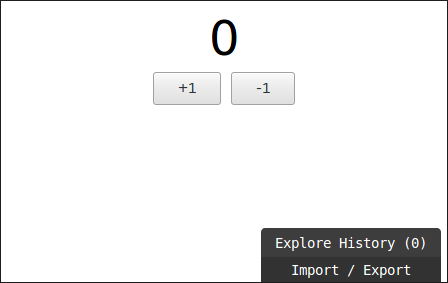
\includegraphics[scale=0.5]{elm-app-sample}
\end{figure}
\end{frame}

\begin{frame}[fragile]
\frametitle{Импорт модулей}
\begin{lstlisting}[language=elm]
module Main exposing (main)

import Html exposing (Html, text, div, button)
import Html.Attributes exposing (class)
import Html.Events exposing (onClick)
\end{lstlisting}
\end{frame}

\begin{frame}[fragile]
\frametitle{Главная функция}
\begin{lstlisting}[language=elm]
main : Program Never Model Msg
main =
    Html.beginnerProgram
        { model = initalModel
        , update = update
        , view = view
        }
\end{lstlisting}
\end{frame}

\begin{frame}[fragile]
\frametitle{Модель}
\begin{lstlisting}[language=elm]
type alias Model =
    { value : Int
    }


initalModel : Model
initalModel =
    { value = 0
    }
\end{lstlisting}
\end{frame}

\begin{frame}[fragile]
\frametitle{Обновление}
\begin{lstlisting}[language=elm]
type Msg
    = Increment
    | Decrement


update : Msg -> Model -> Model
update msg model =
    case msg of
        Increment ->
            { model | value = model.value + 1 }

        Decrement ->
            { model | value = model.value - 1 }
\end{lstlisting}
\end{frame}

\begin{frame}[fragile]
\frametitle{Представление}
\begin{lstlisting}
view : Model -> Html Msg
view model =
    div []
        [ div [ class "counter" ]
            [ text (toString model.value) ]
        , div [ class "controls" ]
            [ button [ onClick Increment ] [ text "+1" ]
            , button [ onClick Decrement ] [ text "-1" ]
            ]
        ]
\end{lstlisting}
\end{frame}

\begin{frame}[fragile]
\frametitle{На стороне HTML}
\begin{lstlisting}[language=HTML]
<script src="/app.js"></script>
<script>
var app = Elm.Main.fullscreen();
</script>
\end{lstlisting}
\end{frame}

\section{Основные инструменты}

\begin{frame}
\frametitle{Установка Elm}
\begin{itemize}
	\item \url{https://guide.elm-lang.org/install.html}
	\item \texttt{npm install -g elm}
	\item \texttt{elm --version}
	\item \texttt{0.18.0}
\end{itemize}
\end{frame}

\begin{frame}
\frametitle{Базовые инструменты Elm}
\begin{itemize}
	\item \texttt{elm-make}
	\item \texttt{elm-package}
	\item \texttt{elm-reactor}
	\item \texttt{elm-repl}
\end{itemize}
\end{frame}

\begin{frame}
\frametitle{Управление пакетами Elm}
\begin{itemize}
	\item \texttt{elm package install elm-community/list-extra}
	\item \url{http://package.elm-lang.org/}
\end{itemize}
\end{frame}

\begin{frame}
\frametitle{Установка и обновление}
\center\texttt{elm package install}

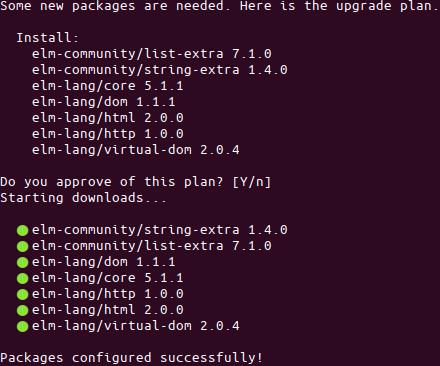
\includegraphics[scale=0.45]{elm-package-install}
\end{frame}

\begin{frame}[fragile]
\frametitle{Файл пакета Elm}
\texttt{elm-package.json}:
\begin{lstlisting}
{
  "version": "1.0.0",
  "summary": "helpful summary of your project, less than 80 characters",
  "repository": "https://github.com/user/project.git",
  "license": "BSD3",
  "source-directories": ["app/elm"],
  "exposed-modules": [],
  "dependencies": {
    "elm-lang/core": "5.0.0 <= v < 6.0.0",
    "elm-lang/dom": "1.1.1 <= v < 2.0.0",
    "elm-lang/html": "2.0.0 <= v < 3.0.0"
  },
  "elm-version": "0.18.0 <= v < 0.19.0"
}
\end{lstlisting}
\end{frame}

\section{Управление кодом на Elm}

\begin{frame}
\frametitle{Brunch}
\begin{itemize}
	\item \texttt{npm install -g brunch}
	\item \texttt{brunch --version}
	\item \texttt{2.10.12}
	\item \texttt{brunch new --skeleton MattCheely/elm-brunch-skeleton demo-application}
	\item \texttt{cd demo-application}
	\item \texttt{npm build}
	\item \texttt{npm start}
\end{itemize}
\end{frame}

\begin{frame}
\frametitle{Отладка}
\begin{figure}
	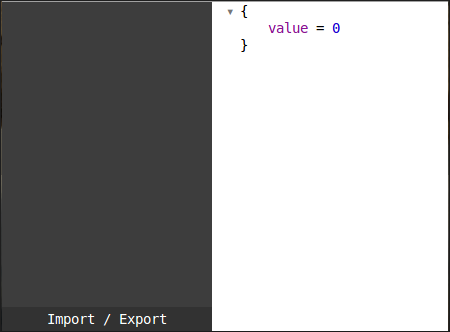
\includegraphics[scale=0.5]{elm-app-sample-state-0}
\end{figure}
\end{frame}

\begin{frame}
\frametitle{Отладка}
\begin{figure}
	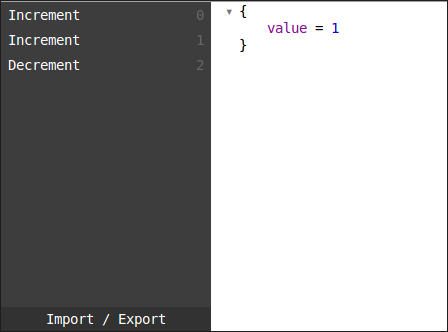
\includegraphics[scale=0.5]{elm-app-sample-state-current}
\end{figure}
\end{frame}

\begin{frame}
\frametitle{Отладка}
\begin{figure}
	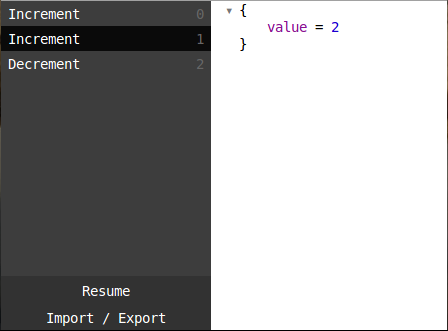
\includegraphics[scale=0.5]{elm-app-sample-state-previous}
\end{figure}
\end{frame}

\section{Дополнительные инструменты}

\begin{frame}
\frametitle{Дополнительные инструменты}
\begin{itemize}
	\item \textit{\texttt{elm-format}} \url{https://github.com/avh4/elm-format}
	\item \textit{\texttt{elm-format-short}} \url{https://github.com/nukisman/elm-format-short}
	\item \textit{\texttt{elm-analyse}} \url{https://www.npmjs.com/package/elm-analyse}
\end{itemize}
\end{frame}

\begin{frame}
\frametitle{elm-analyse: главное окно}
\center\texttt{elm-analyse -s}

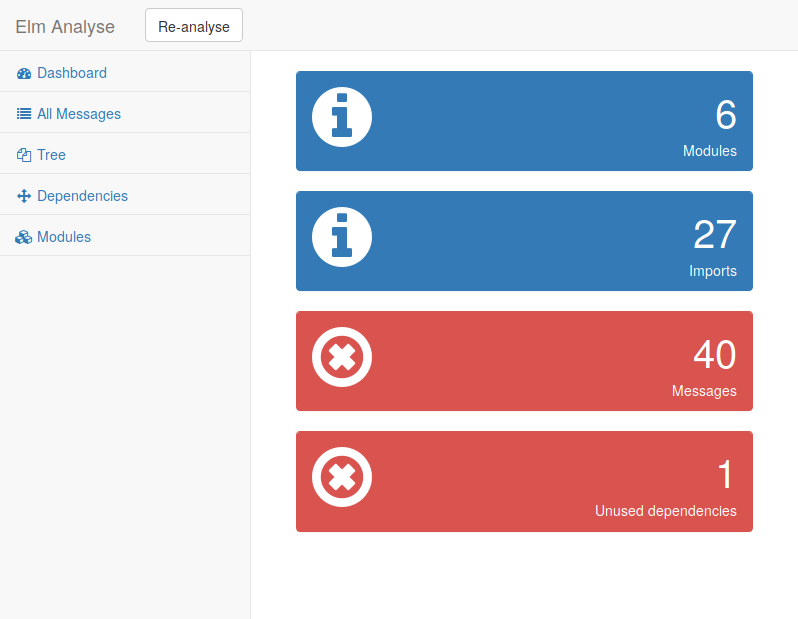
\includegraphics[scale=0.3]{elm-analyse-in-browser-main}
\end{frame}

\begin{frame}
\frametitle{elm-analyse: список проблем}
\center\texttt{elm-analyse -s}

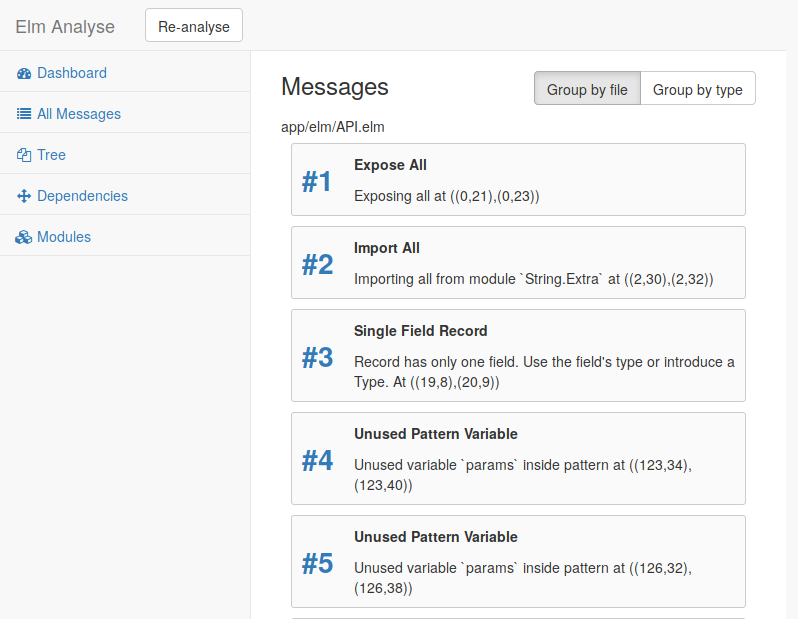
\includegraphics[scale=0.3]{elm-analyse-in-browser-problems}
\end{frame}

\begin{frame}
\frametitle{elm-analyse: пример с фрагментом кода}
\center\texttt{elm-analyse -s}

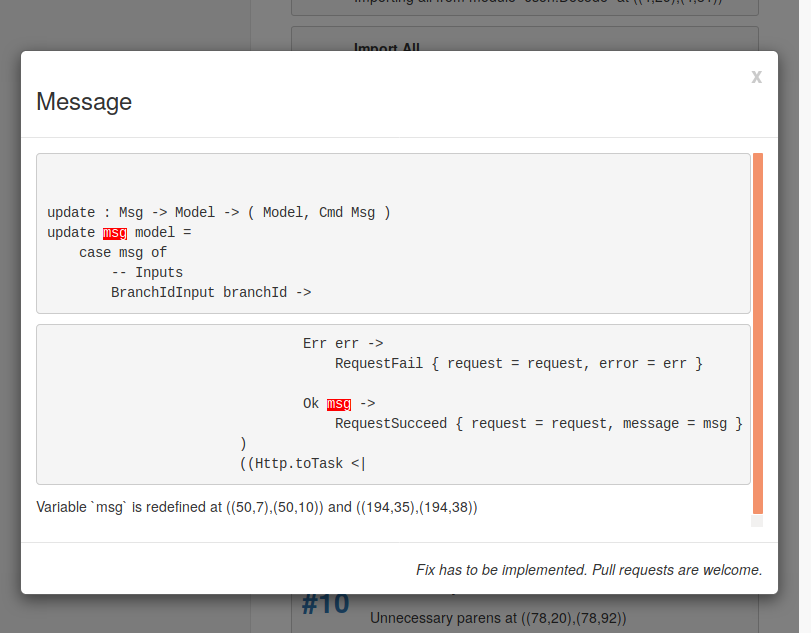
\includegraphics[scale=0.3]{elm-analyse-in-browser-redefine-sample}
\end{frame}

\section{Среды разработки}

\begin{frame}
\frametitle{Среды разработки}
\begin{itemize}
	\item Atom \url{https://habr.com/post/347730/}
	\item Light Table \url{https://habr.com/post/302154/}
	\item Visual Studio Code
	\item GNU Emacs
	\item другие
\end{itemize}
\end{frame}

\begin{frame}
\frametitle{Настройка Atom для работы с Elm}
\begin{itemize}
	\item \texttt{language-elm}
	\item \texttt{atom-ide-ui}
	\item \texttt{autocomplete-plus}
	\item \texttt{elmjutsu}
	\item \texttt{elm-format}
	\item \texttt{linter}
	\item \texttt{linter-elm-make}
	\item \texttt{elm-lens}
	\item \texttt{elm-instant}
	\item \texttt{platformio-ide-terminal}
\end{itemize}
\end{frame}

\begin{frame}
\frametitle{Atom в процессе работы с Elm}
\begin{figure}
	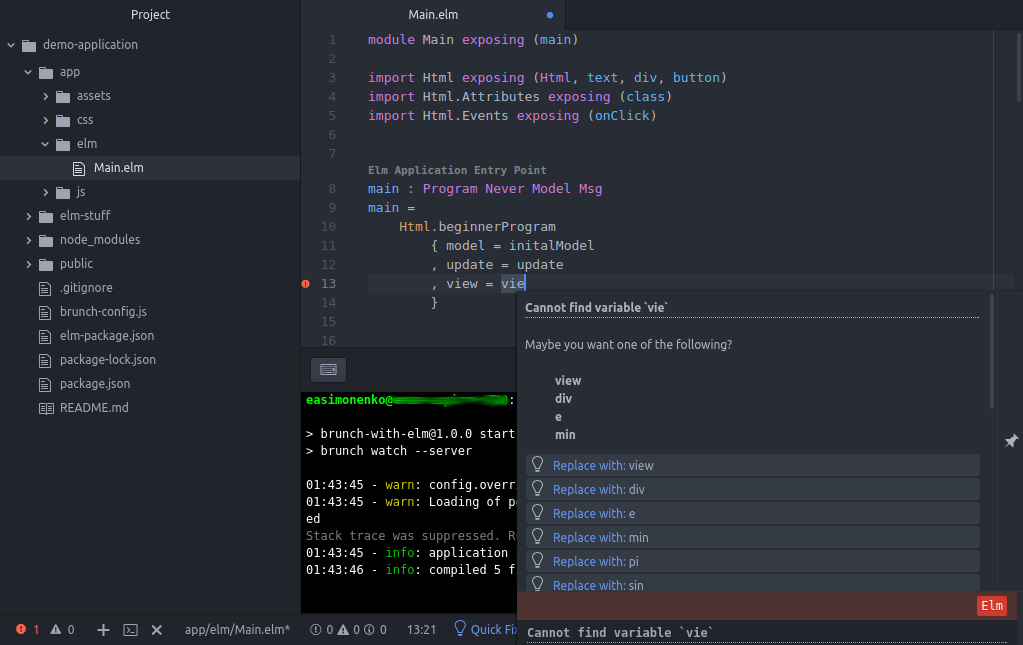
\includegraphics[scale=0.3]{elm-code-in-atom-with-error}
\end{figure}
\end{frame}

\section{Интероперабельность}

\begin{frame}
\frametitle{Способы интероперабельности}
\begin{itemize}
	\item port
	\item native module
\end{itemize}
\end{frame}

\begin{frame}[fragile]
\frametitle{Пример с port (код на Elm)}
\begin{lstlisting}[language=elm]
port title : String -> Cmd msg
...
title <| "Site Title :: " ++ pageTitle
\end{lstlisting}
\end{frame}

\begin{frame}[fragile]
\frametitle{Пример с port (код на JavaScript)}
\begin{lstlisting}
app.ports.title.subscribe(function (title) {
  document.title = title;
});
\end{lstlisting}
\end{frame}

\section{За и против, и что в будущем}

\begin{frame}
\frametitle{Результат опроса}
\url{https://habr.com/post/347730/}
\begin{itemize}
	\item не нужен в принципе: 26.9\%
	\item годный, но на нём не пишу: 25\%
	\item в первый раз вижу, но выглядит годным: 19.2\%
	\item сыроват для серьёзной разработки: 15.3\%
	\item годный, я на нём уже программирую: 13.4\%
\end{itemize}
\end{frame}

\begin{frame}
\frametitle{За Elm}
Технические ``за'':
\begin{itemize}
	\item если скомпилировалось, то и работать будет
	\item отсутствие исключений и неопределённостей
	\item более понятная последовательная логика
	\item более простой и ясный синтаксис
\end{itemize}

Социальные ``за'':
\begin{itemize}
	\item ???
\end{itemize}
\end{frame}

\begin{frame}
\frametitle{Против Elm}
Технические ``против'':
\begin{itemize}
	\item сложный механизм интероперабельности
	\item недостаточный спектр прикладных пакетов
	\item большой объём скомпилированного кода
	\item отсутствие модульности во время исполнения
	\item несовместимость кода для разных версий компилятора
\end{itemize}

Социальные ``против'':
\begin{itemize}
	\item необходимость переключиться в иную парадигму
	\item практически полное отсутствие кадров
	\item мало историй успеха
	\item отсутствие поддержки со стороны компаний
	\item неясность перспективы
\end{itemize}
\end{frame}

\begin{frame}
\frametitle{Что в будущем}

\begin{itemize}
	\item совершенствование инструментов разработчика
	\item улучшение поддержки разработки SPA
	\item не планируется поддержка других платформ
\end{itemize}

Подробности: \url{https://github.com/elm-lang/projects/blob/master/roadmap.md}

\end{frame}

\section{Что почитать}

\begin{frame}
\frametitle{Что почитать}
\begin{itemize}
	\item \url{https://habr.com/post/347730/}
	\item \url{https://habr.com/post/347730/}
	\item \url{http://ts-soft.ru/blog/elm-part-1}
	\item \url{http://ts-soft.ru/blog/elm-part-2}
	\item \url{https://habr.com/hub/elm/}
	\item \url{http://elm-lang.org/docs}
\end{itemize}
\end{frame}

\section{Ссылки}

\begin{frame}
\frametitle{Ссылки}
\begin{itemize}
\item \url{http://elm-lang.org/}
\item \url{http://brunch.io/}
\item \url{https://github.com/halohalospecial/atom-elmjutsu}
\item \url{https://github.com/avh4/elm-format}
\item \url{https://vk.com/elm_lang_ru}
\end{itemize}
\end{frame}

\section*{Благодарность}

\begin{frame}
\center

\textit{Благодарю за внимание!}

\textbf{\textsl{\inserttitle}}

\insertauthor
\end{frame}
\end{document}
